\documentclass[12pt]{scrartcl}
\usepackage{fullpage,enumitem,amsmath,amssymb,graphicx,color}

\addtokomafont{section}{\normalsize}
\setlength{\parindent}{0pt}

\newcommand{\vect}[1]{\boldsymbol{#1}}
\newcommand{\ve}{\vect}
\newcommand\R{\mathbb{R}}
\newcommand\E{\mathbb{E}}
\newcommand{\fx}[1]{#1(\vect{x})}
\newcommand{\diff}[1]{\,\mathrm{d}#1}

\title{\large Machine Learning Exercise Sheet 2}
\subtitle{\Large k-Nearest Neighbors and Decision Trees}
\author{\large\bfseries Group\_369 \\
        \large Fan \textsc{Xue} -- \texttt{fan98.xue@tum.de} \\
        \large Xing \textsc{Zhou} -- \texttt{xing.zhou@tum.de} \\
        \large Jianzhe \textsc{Liu} -- \texttt{jianzhe.liu@tum.de}}
\date{\large \today}
\begin{document}


  \maketitle
  \vspace{-1cm}
  \noindent\rule{\textwidth}{0.4pt}
 
  
  \section*{Problem 1}

According to the question we have:
\\
\\
A(1, 1)\quad B(2, 0.5)\quad C(1, 2.5)\quad D(3, 3.5)\quad E(5.5, 3.5)\quad F(5.5, 2.5)

    \begin{enumerate}[label=\alph*)]
      \item 
According to $L_1-$Norm,
\[d_1(X, Y) = \sum_{i}\lvert X_i - Y_i \rvert\]
we have for example:
\[d_{AB} = \lvert 1 - 2 \rvert + \lvert 1 - 0.5 \rvert = 1.5\]     
By using this formula we can compute every distance between each two points and fill the results in a table:
\begin{table}[h!]
  \begin{center}
    \begin{tabular}{c|c|c|c|c|c|c|c|c} % <-- Alignments: 1st column left, 2nd middle and 3rd right, with vertical lines in between
      \textbf{$L_1-$Norm} & \textbf{A} & \textbf{B} & \textbf{C} & \textbf{D} & \textbf{E} & \textbf{F} & \textbf{N-Neighbor} & \textbf{Class}\\
      \hline
      \textbf{A} & 0.0 & \color{red}1.5 & \color{red}1.5 & 4.5 & 7.0 & 6.0 & B or C & 1\\
      \textbf{B} & \color{red}1.5 & 0.0 & 3.0 & 4.0 & 6.5 & 5.5 & A & 1\\
      \textbf{C} & \color{red}1.5 & 3.0 & 0.0 & 3.0 & 5.5 & 4.5 & A & 1\\
      \textbf{D} & 4.5 & 4.0 & 3.0 & 0.0 & \color{red}2.5 & 3.5 & E & 2\\
      \textbf{E} & 7.0 & 6.5 & 5.5 & 2.5 & 0.0 & \color{red}1.0 & F & 2\\
      \textbf{F} & 6.0 & 5.5 & 4.5 & 3.5 & \color{red}1.0 & 0.0 & E & 2\\
    \end{tabular}
  \end{center}
\end{table}

We can see that with leave-one-out cross validation, all the points are correctly classified.
     \item 
According to $L_2-$Norm,
\[d_2(X, Y) = \left( \sum_{i}(X_i - Y_i)^2 \right)^{\frac{1}{2}}\]
we have for example:
\[d_{AB} = \left((1 - 2) + (1 - 0.5)\right)^{\frac{1}{2}} = 1.118 \approx 1.2\]  
Same as before, we still can use this formula to compute every distance between each two points and fill the results in another table:
\begin{table}[h!]
  \begin{center}
    \begin{tabular}{c|c|c|c|c|c|c|c|c} % <-- Alignments: 1st column left, 2nd middle and 3rd right, with vertical lines in between
      \textbf{$L_1-$Norm} & \textbf{A} & \textbf{B} & \textbf{C} & \textbf{D} & \textbf{E} & \textbf{F} & \textbf{N-Neighbor} & \textbf{Class}\\
      \hline
      \textbf{A} & 0.00 & \color{red}1.12 & 1.50 & 3.20 & 5.15 & 4.74 & B & 1\\
      \textbf{B} & \color{red}1.12 & 0.00 & 2.24 & 3.16 & 4.61 & 4.03 & A & 1\\
      \textbf{C} & \color{red}1.50 & 2.24 & 0.00 & 2.24 & 4.61 & 4.50 & A & 1\\
      \textbf{D} & 3.20 & 3.16 & \color{red}2.24 & 0.00 & 2.50 & 2.69 & C & \color{blue}1\\
      \textbf{E} & 5.15 & 4.61 & 4.61 & 2.50 & 0.00 & \color{red}1.00 & F & 2\\
      \textbf{F} & 4.74 & 4.03 & 4.50 & 5.69 & \color{red}1.00 & 0.00 & E & 2\\
    \end{tabular}
  \end{center}
\end{table}

We can see that when we use $L_2-$Norm to validate our data, an error occurs: Point D is classified as Class 1 instead of 2.
     \item
According to these two cases we can draw the conclusion that a point can be classified into different class if we use different distance measurement. In our case, point D is close to Class 2 in the view of $L_1-$Norm yet close to Class 1 in the view of $L_2-$Norm.
\end{enumerate}

  \section*{Problem 2}
 
\begin{enumerate}[label=\alph*)]
    \item 
If we use unweighted K-NN and $K_{new} = N_A + N_B + N_C$, then for $X_{new}$, the result would definitely be \textbf{Class C}. Because K-NN algorithm will always classify the new data into its major neighbor's class. If we use K that concludes every data in this training set, then the majority of the classes are equal to the major neighbors.
    \item
If we use weighted K-NN, whether the problem would be solved remains uncertain. If some cases it may, but in our case, we are lacking further information about our data's feature, thus not being able to conduct further calculations.
\end{enumerate}  
  
  \section*{Problem 3}


    \begin{enumerate}[label=\alph*)]
      \item 
After observing this training model we can find that each data in this model has many features, and those features has huge differences on ranges. So if this model performs bad on test set, the reason could be followings:
\begin{enumerate}[label=\arabic*.]
\item
Those features in different ranges have different impact on the result. Solution should be: Using data Standardization:
\[x^{'}_{i} = \frac{x_i - \mu_i}{\sigma_i}   \]
or Mahalanobis distance:
\[ \sqrt{(\textbf{u}-\textbf{v})^T\Sigma^{-1}(\textbf{u}-\textbf{v})}\]
\item
Considering so many data, the choice of K can also affect the final result. Solution to this point is simple, we should use various K on validation set and find a better K for this model.
\item
Still, when there are so many data, it's possible that a shift occurs between the training set and the test set. For example, in the training set there are only few samples about vans yet in the test set the majority of the samples are vans. Solution to this would be, equally divide the samples into different set to make minimize the shift.
\item
When there are too many features in a single sample, it would bring the curse of dimension, which will lead to the lack of samples. As a result, the distance between samples will be amplified, and this could cause bad performance on test set. We can only use another algorithm to try to minimize this problem but we can't solve it so far. 
\end{enumerate} 
\item
If we use decision tree, the above-mentioned problems would be:
\begin{enumerate}[label=\arabic*.]
\item
Features in different ranges will no longer affect the result, because in each node of the decision tree, only one feature will be discussed, that is to say, the other feature will have no impact on this exact node.
\item
I would say, the parameter K in K-NN algorithm is just like the way we divide the decision trees. In K-NN, we can use some methods to find a better K, here in DT, we can also find a better way to divide the nodes, by using Misclassification rate, entropy or Gini index.
\item
The shift on both sets also exists here and the solution is almost the same.
\item
As said above, the curse of dimension will always more or less affect the result.
\end{enumerate}
\end{enumerate} 
  \section*{Problem 4}  

Can be \textbf{proved} by:
\begin{equation*}
  \begin{aligned}
    d_1(x, y)^2 &= \left( \sum_{i}\lvert X_i - Y_i \rvert \right)^2 \\
                &= \sum_{i}(X_i - Y_i)^2 + 2\sum_{i}\sum_{j, j \neq i} \lvert X_i - Y_i \rvert\lvert X_j - Y_j \rvert\\
                &\geq \sum_{i}(X_i - Y_i)^2 \\
                &=d_2(x, y)^2\
  \end{aligned}
\end{equation*}
Since $d_1$ and $d_2$ are all $>0$, we can draw the conclusion that:
\[d_1(x, y) \geq d_2(x, y)\]
  \section*{Problem 5}
 
Can be \textbf{disproved} by following example:
\\
\\
Assuming that we have 3 different points:\quad $y$(2, 2) \quad $x_1$(1, 0.5) \quad $x_2$(2, 0)
\\
\\
In $L_2-$Norm we have:
\[ d_2(y, x_1) = \sqrt{(2-1)^2 + (2-0.5)^2} = 1.803 \approx 1.8    \]
\[ d_2(y, x_2) = \sqrt{(2-2)^2 + (2-0)^2} = 2     \]
Obviously we have: $d_2(y, x_1) < d_2(y, x_2)$.
\\
\\
Let's say we only have these 3 points, then 
$x_1$ is the nearest neighbor of $y$ in $L_2-$Norm.
\\
\\
But in $L_1-$Norm we have:
\[ d_1(y, x_1) = \lvert 2 - 1 \rvert + \lvert 2 - 0.5 \rvert = 2.5    \]
\[ d_1(y, x_2) = \lvert 2 - 2 \rvert + \lvert 2 - 0 \rvert = 2    \]
Obviously we have: $d_1(y, x_1) > d_1(y, x_2)$.
\\
\\
That is to say, in $L_1-$Norm, $x_1$ isn't the nearest neighbor of $y$.

\section*{Problem 6}

  Yes. We can define two new features $y_1 = x_1 - x_2$ and $y_2 = x_2$. By doing 
  this, we can split the dataset by judging the condition $y_1 \leqslant 0$. With
  only one split the dataset is split into two parts and each part only has one sort
  of class. It means, there exists a decision tree of depth 1 that classifies this 
  dataset with 100\% accuracy.

  
  \section*{Problem 7}
    \begin{enumerate}[label=\alph*)]
      \item 
      \begin{equation*}
        \begin{split}
          i_H(y) &= -p(y=W)\log{p(y=W)} - p(y=L)\log{p(y=L)}  \\
          &= -\frac{4}{10}\log{\frac{4}{10}} - \frac{6}{10}\log{\frac{6}{10}} \\
          &= 0.971
        \end{split} 
      \end{equation*}
      \item 
      Splitting by \(x_1 = T\) \\
      \[
        \begin{split}
          \Delta i_H &= i_H(y) - p(x_1 = T)i_H(x_1=T) - p(x_1=I)i_H(x_1=I) \\
          &= 0.971 - \frac1 2( -\frac2 5\log{\frac2 5} - \frac3 5\log{\frac3 5} ) 
          -\frac1 2( -\frac2 5\log{\frac2 5} - \frac3 5\log{\frac3 5} ) \\
          &= 0
        \end{split}
      \]
      Splitting by \(x_2 = M\) \\
      \[
        \begin{split}
          \Delta i_H &= i_H(y) - p(x_2 = M)i_H(x_1=M) - p(x_2=P)i_H(x_2=P) \\
          &= 0.971 - \frac4 {10}( -\frac2 4\log{\frac2 4} - \frac2 4\log{\frac2 4} ) 
          -\frac6 {10}( -\frac2 6\log{\frac2 6} - \frac4 6\log{\frac4 6} ) \\
          &= 0.020
        \end{split}
      \]
      Splitting by \(x_3 = S\) \\
      \[
        \begin{split}
          \Delta i_H &= i_H(y) - p(x_3 = S)i_H(x_3=S) - p(x_3=C)i_H(x_3=C) \\
          &= 0.971 - \frac1 2( -\frac3 5\log{\frac3 5} - \frac2 5\log{\frac2 5} ) 
          -\frac1 2( -\frac1 5\log{\frac1 5} - \frac4 5\log{\frac4 5} ) \\
          &= 0.125
        \end{split}
      \]
      According to the calculation the split judgement will be \(x_3 = S\), since
      in this case, the \(\Delta i_H\) is the biggest. If \(x_3 = S\), the instance
      will be classified as W. Otherwise it will be classified as L.
    \end{enumerate}
\clearpage    
  \section*{Problem 8}
  Let \(i^2 = \frac{125}{i}\), we get \(i = 5\). Figure 1 shows the 2-d space of the
  dataset. 
  \begin{figure}[!htb] %H为当前位置,!htb为忽略美学标准,htbp为浮动图形
    \centering %图片居中
    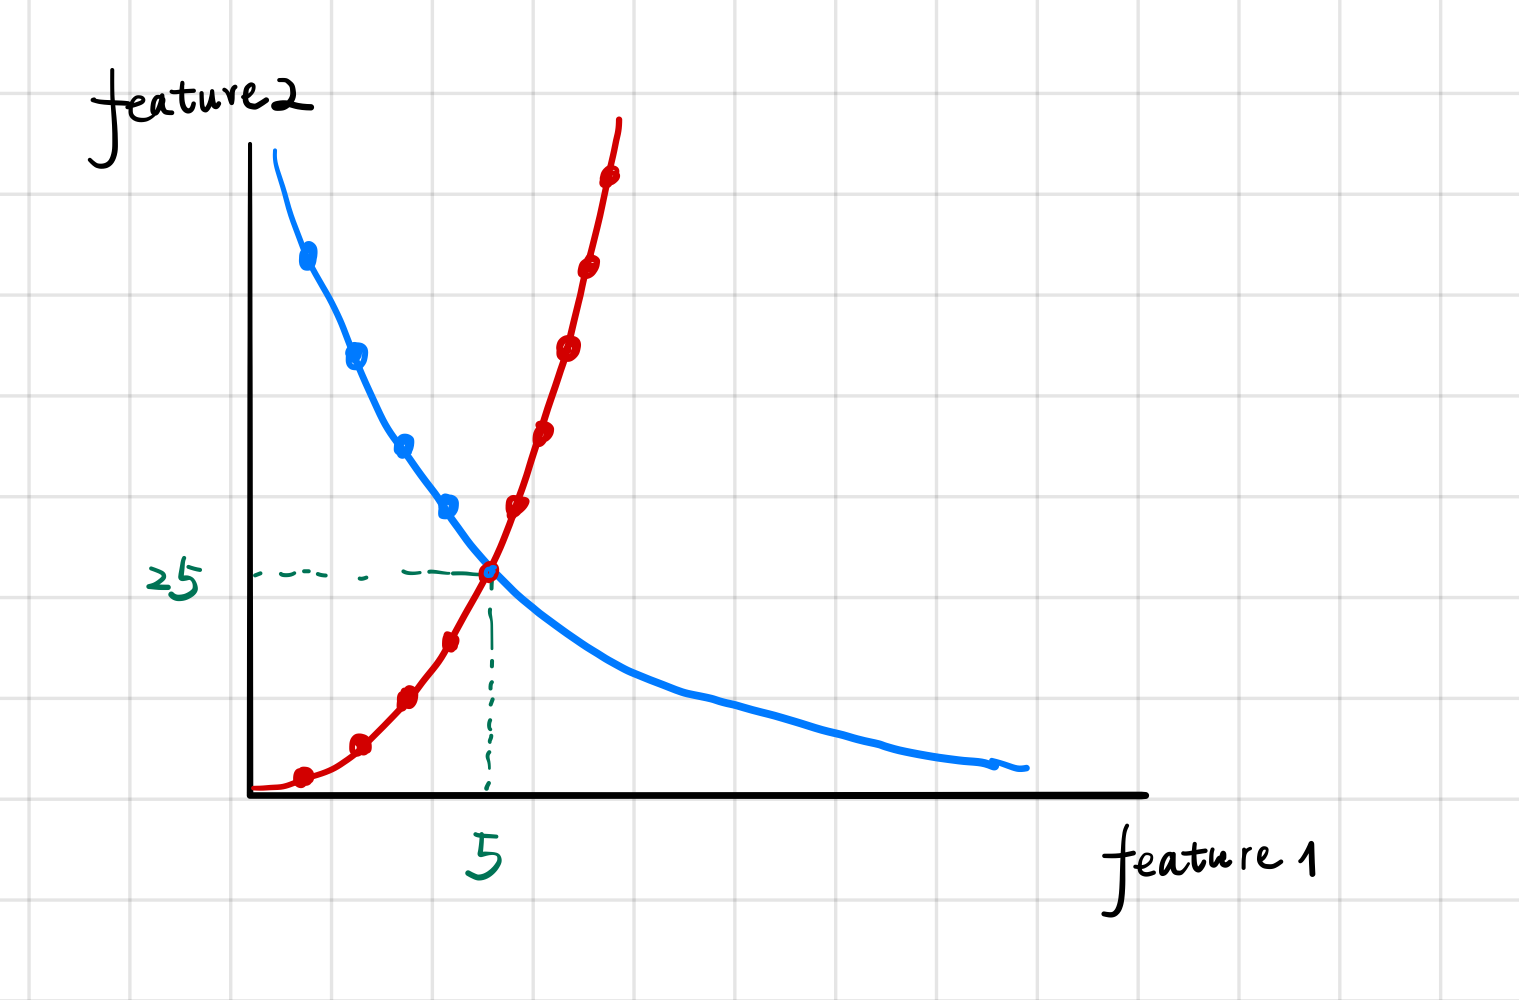
\includegraphics[width=0.7\textwidth]{Problem8.png} %插入图片,[]中设置图片大小,{}中是图片文件名
    \caption{the 2-d space of the dataset} %最终文档中希望显示的图片标题
    \label{Fig.main2} %用于文内引用的标签
  \end{figure}
  
  We can easily split the dateset into 4 parts.
  The first split uses the threshold \(\text{feature2} \leqslant 25\). \\
  The second split uses the threshold \(\text{feature1} \leqslant 5\) for both child nodes. \\
  In this way, the depth of the decision tree is 2. Only one datapoint (5, 25) is missclassified,
  which is unavoidable.
  
    \section*{Problem 9}
 
 The result of programming will be shown in next few pages.
  
\end{document}